\section{Реализация инструмента для анализа обменов на шине I2C}

\label{implementation}

В рамках курсовой работы стояла задача по реализации инструмента для анализа обменов на шине I2C на базе уже существующего решения для визуализации и анализа обменов Opermon. В этом разделе описаны детали реализации решения.

\subsection{Выбор адаптера}

Для получения данных с шины I2C был выбран адаптер Bus Pirate [\ref{buspirate_descr}] по следующим причинам:

\begin{itemize}
 \item Адаптер имеет простой и удобный интерфейс взаимодействия, как консольный (для работы без специализированного ПО), так и бинарный;
 \item Bus Pirate поддерживает режим I2C sniffer [\ref{buspirate_i2c}], что необходимо для реализации средства анализа;
 \item Bus Pirate - проект с открытым исходным кодом и открытой реализацией оборудования. Вокруг проекта образовалось обширное сообщество, постоянно занимающееся разработкой новых версий аппаратного и программного обеспечения;
 \item Доступная стоимость адаптера.
\end{itemize}

Сообщения в формате Bus Pirate (в бинарном режиме) имеют текстово-бинарный формат (отдельно кодируются символы, обозначающие события на шине). Данные об обменах представляются в следующем виде [\ref{buspirate_i2c_snif}]:

\begin{itemize}
 \item символ ``\textbf{[}'' обозначает начало обмена (событие \textbf{START});
 \item символ ``\textbf{]}'' обозначает конец сообщения (событие \textbf{STOP});
 \item ответы принимающей стороны - \textbf{ACK} и \textbf{NACK} кодируются символами ``\textbf{+}'' и ``\textbf{-}'' соответственно;
 \item передаваемые данные начинаются с символа ``\textbf{\textbackslash}'', после чего cледует считанный байт данных.
\end{itemize}

Пример фрагмента получаемого потока данных от адаптера (\\0xMN - бинарное значение, 1 байт):

\begin{verbatim}
 [\\0xA0+\\0x01+\\0x02+][\\0xA1+\\0xDE+\\0xAD+\\0xF0+\\0x0D-]
\end{verbatim}

\subsection{Проектирование решения}

\subsubsection{Серверная часть}

Задача удалённого агента - определять подключенные к системе совместимые адаптеры и осуществлять обмен данными между Opermon и выбранным адаптером. Обмен с адаптером происходит посредством последовательного соединения.

Алгоритм поиска доступных в системе адаптеров приведён на схеме ниже. С помощью такого алгоритма можно определить также устройства, совместимые с Bus Pirate. При проверке адаптер только переводится в режим бинарного интерфейса, что безопасно для подключенного оборудования. После проверки обнаруженные адаптеры перезапускаются для того, чтобы оставить пользователю возможность использовать часть адаптеров в режиме консольного интерфейса.

\begin{figure}[H]
 \centering
 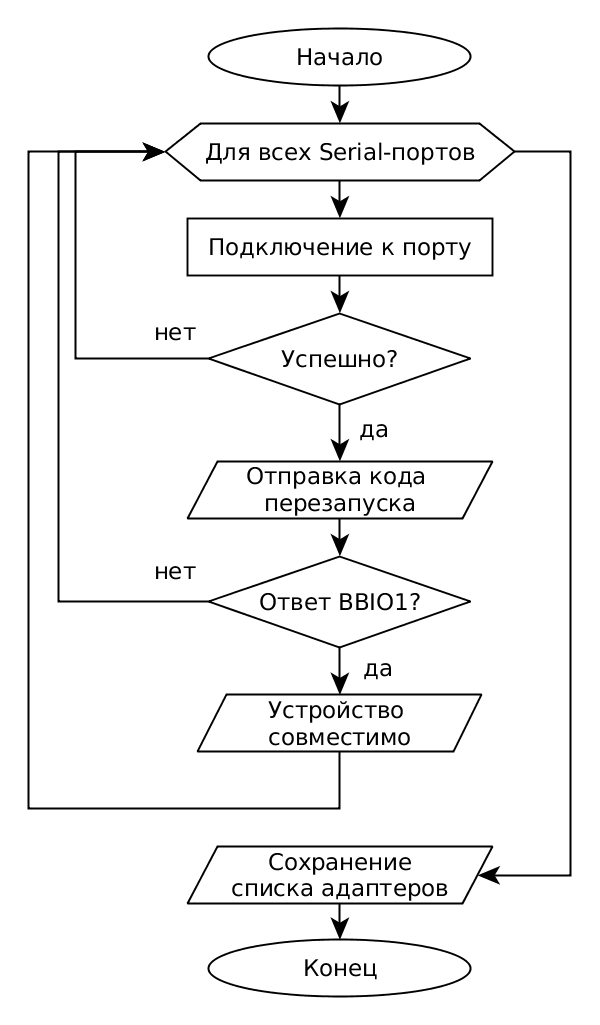
\includegraphics[width=0.5\textwidth]{bp-discovery}
 \caption{Алгоритм обнаружения Bus Pirate - совместимых адаптеров в системе}
 \label{fig:bp-discovery}
\end{figure}

Добавление нового адаптера в серверную часть означает следующую последовательность действий:

\begin{enumerate}
 \item добавление класса (C++), соответствующего типу адаптера, а также реализация в нём методов для управления адаптером, список которых приведён в разделе \ref{agent_proc_list};
 \item добавление создания экземпляра класса и вызовов методов в процедуру обработки RPC-запросов;
 \item реализация процедуры получения и сериализации данных от адаптера для передачи их клиентской части.
\end{enumerate}

\subsubsection{Клиентская часть}

В клиентской части требуется проводить разбор сообщений из данных, приходящих от Bus Pirate, во внутренние представления Opermon, а также реализовать необходимые виджеты для отображения данных и настройки параметров. 

Добавление нового типа адаптера в Opermon означает следующую последовательность действий:

\begin{enumerate}
 \item описание нового типа обменов в компоненте Tabexchange;
 \item описание нового типа представления адаптера в клиентской части;
 \item реализация процедуры получения данных от серверной части и создание экземпляров нового типа обменов на их базе;
 \item добавление создания экземпляра класса представления адаптера в соответствующую процедуру в Opermon;
 \item реализация необходимых для работы виджетов на базе предлагаемых в решении интерфейсов в компоненте sma;
 \item добавление создания экземпляров классов виджетов и код для их базовой настройки в фабрику виджетов.
\end{enumerate}


\subsection{Добавление поддержки адаптера в Opermon}

\subsubsection{Серверная часть}

\label{server_implementation}

Серверная часть решения реализована с использованием библиотеки QSerialPort [\ref{qtserialport}] для упрощения работы с последовательным интерфесом адаптера.

Для реализации поддержки адаптера на стороне сервера были выполнены следующие действия:

\begin{itemize}
 \item Создана обёртка для библиотеки QSerialPort для сборки в рамках системы сборки cvslvk.
 \item Описан класс BusPirate представления адаптера, наследуемый от класса CommonCard. В базовом классе реализованы основные функции представления адаптера, такие как установление TCP-соединения с клиентской частью, проверка наличия новых данных по файловому дескриптору и т.д. В классе BusPirate реализованы методы для инициализации последовательного порта, конфигурирования адаптера и получения данных от адаптера с выделением отдельных обменов.
 \item В обработчик RPC-запросов RpcServer::processRequest() добавлено создание объекта представления адаптера и вызовы соответствующих методов.
\end{itemize}


\subsubsection{Клиентская часть}

\label{client_implementation}

Для реализации поддержки адаптера на клиентской стороне были выполены следующие действия:

\begin{itemize}
 \item Описано представление обмена в Tabexchange. Для этого создан класс BPI2CExchange, наследуемый от Exchange. Каждый обмен в среде Opermon представлен в виде экземпляра этого класса, при этом в базовом классе Exchange реализуется работа с параметрами обмена, общими для разных типов адаптеров (такие как время получения, порядковый номер обмена и т.д.), в классе BPI2CExchange реализуется разбор обмена из полученных ``сырых'' данных от адаптера и хранение отдельных полей обмена: адреса slave-устройства, режима доступа и полезной нагрузки.
 \item Описано представление адаптера и реализован интерфейс взаимодействия с серверной частью в Opermon. Для этого создан класс BPI2CMTCard, наследуемый от OperMon::CommonCard. В базовом классе реализуется идентификация конкретного адаптера, проверка соединения с представлением адаптера на удалённом агенте, а также вызовы основных методов в RPC. В классе BPI2CMTCard дополнительно реализуется начальная конфигурация адаптера на удалённом агенте и разбор полученных данных с выделением обменов. Передача нового полученного обмена в обработку в среде Opermon происходит через Qt-сигнал addExchange(Exchange *).
 \item Реализовано представление адаптера в пользовательском интерфейсе в классе BPI2CChannelInfo, наследуемом от ChannelInfo. Представление реализует настройку параметров адаптера: в базовом классе реализуется настройка соединения с удалённым агентом (адрес хоста, номер адаптера в системе и т.д.), в наследнике реализуется тип роли адаптера (на сегодняшний день только чтение канала - Sniffer) и настройка параметров, специфичных для адаптера (включение питания целевого устройства, резисторы подтяжки и т.д.).
 \item Добавлено значение BPI2CChannel в список типов адаптеров в ChannelType.
 \item Реализованы классы виджетов для отображения данных обменов и настройки параметров в sma: BPI2CExchangeDetails, BPI2CExchangeInfo, BPI2CExchangeTableModel, BPI2CExchangeTab, BPI2CChannelAttributeModel  и т.д. (с соответствующими базовыми классами ExchangeDetails, ExchangeInfo, ExchangeTableModel, ExchangeTab, ChannelAttributeModel и т.д.).
 \item Добавлено создание экземпляров классов виджетов и их начальная настройка в фабрику виджетов (в sma в класс ChannelFactoryImpl, реализующий интерфейс ChannelFactory).
\end{itemize}


Снимок экрана с окном получившегося интерфейса можно посмотреть в приложении \ref{app:figures} на рисунке \ref{fig:opermon}.